\newpage
\subsection*{\underline{WKB Approximation}}
\begin{figure}[h]
	\centering
	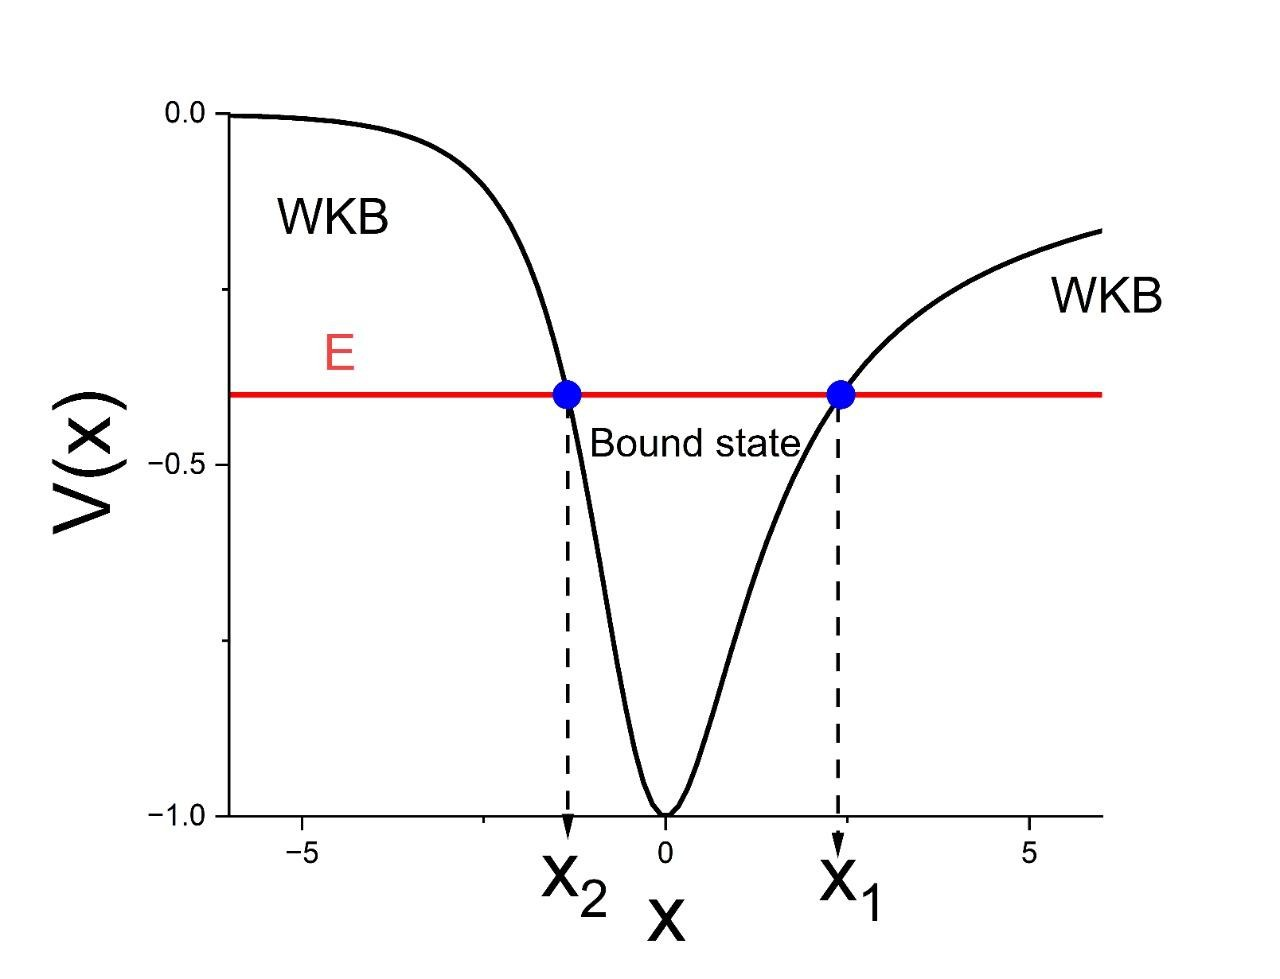
\includegraphics[width=0.5\linewidth]{./figures/wkb-bound-states.png}
	\caption{WKB Bound States}
	\label{fig:wkb-bound-states}
\end{figure}
\begin{align}
	p(x) \equiv \sqrt{2m[E-V(x)]}
\end{align}
\begin{align}
	\psi(x) \approx \frac{C}{\sqrt{p(x)}} \, e^{\pm \frac{i}{\hbar} \int p(x)\, dx}
	%\qquad \psi(x) \approx \frac{C}{\sqrt{|p(x)|}} \, e^{\pm \frac{i}{\hbar} \int |p(x)|\, dx}
	\qquad; \quad E > V
\end{align}
\begin{align}
	\psi(x) \approx \begin{cases}
		\frac{C_1}{\sqrt{p(x)}} \sin{\left[ \frac{1}{\hbar} \int_{x_1}^{x} p(x')\, dx' + \frac{\pi}{4}\right]}, & x_1<x ; \\
		\frac{C_2}{\sqrt{p(x)}} \sin{\left[ \frac{1}{\hbar} \int_{x}^{x_2} p(x')\, dx' + \frac{\pi}{4}\right]}, & x<x_2 
	\end{cases}
\end{align}
Potential well with no vertical walls
\begin{align}
	\int_{x_1}^{x_2} p(x) \, dx = \left( n - \frac{1}{2} \right) \pi \hbar
\end{align}
Potential well with one vertical wall
\begin{align}
	\int_0^{x_2} p(x)\, dx = \left(n - \frac{1}{4} \right) \pi \hbar
\end{align}
Potential well with two vertical walls
\begin{align}
	\int_0^a p(x) \, dx = n\pi \hbar
\end{align}




\newpage
\begin{figure}[h]
	\centering
	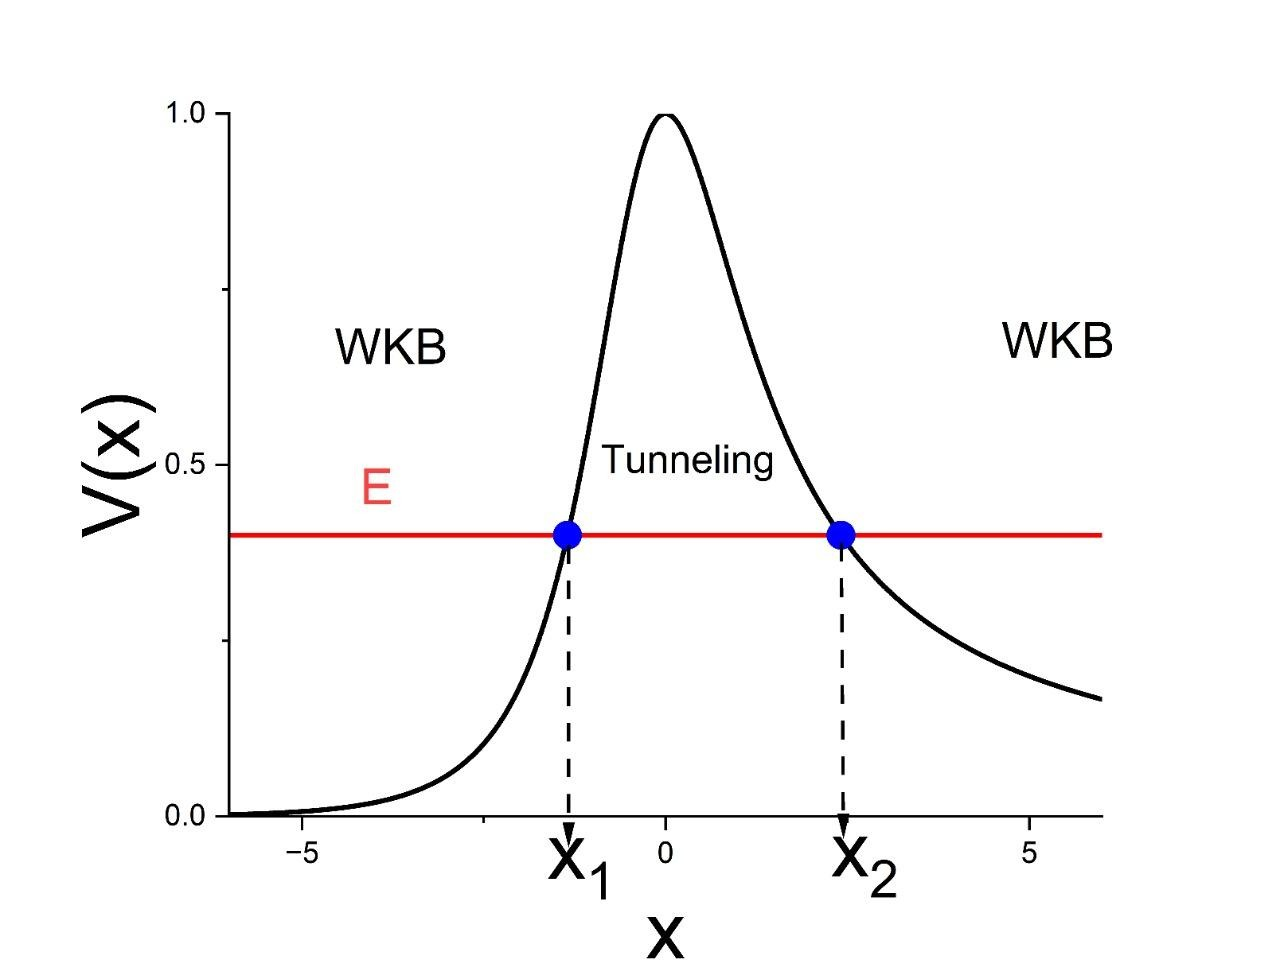
\includegraphics[width=0.5\linewidth]{./figures/wkb-tunneling.png}
	\caption{WKB Tunneling}
	\label{fig:wkb-tunneling}
\end{figure}
\begin{align}
	K(x) \equiv \sqrt{2m[V(x)-E]}
\end{align}
\begin{align}
	\psi(x) \approx \frac{C}{\sqrt{K(x)}} \, e^{\pm \frac{1}{\hbar} \int K(x)\, dx}
	\qquad; \quad E < V
\end{align}
\begin{align}
	\psi(x) \approx \begin{cases}
		\frac{C_1}{\sqrt{K(x)}} \exp{\left[- \frac{1}{\hbar} \int_{x_1}^{x} K(x')\, dx' \right]}, & x>x_1;\\
		\frac{C_2}{\sqrt{K(x)}} \exp{\left[- \frac{1}{\hbar} \int_{x}^{x_2} K(x')\, dx' \right]}, & x<x_2.
	\end{cases}
\end{align}
 

%\begin{align}
%	\psi(x) \approx \frac{C}{\sqrt{p(x)}} \, e^{\pm \frac{i}{\hbar} \int p(x)\, dx}
%	\qquad \psi(x) \approx \frac{C}{\sqrt{|p(x)|}} \, e^{\pm \frac{i}{\hbar} \int |p(x)|\, dx}; \quad E < V
%\end{align}
\begin{align}
	T \sim e^{-2 \gamma}, \qquad \gamma \equiv \frac{1}{\hbar} \int_0^a K(x)\, dx
\end{align}
\newpage
\begin{figure}[h]
	\centering
	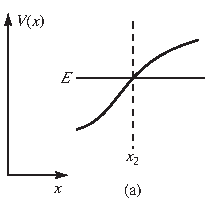
\includegraphics[width=0.3\linewidth]{./figures/right-turning-point.pdf}
	\caption{Right Turning Point}
	\label{fig:right-turning-point}
\end{figure}
\begin{align}
	\psi(x) \approx \begin{cases}
		\frac{2D}{\sqrt{p(x)}} \sin{\left[ \frac{1}{\hbar} \int_{x}^{x_2} p(x')\, dx' + \frac{\pi}{4}\right]}, & x<x_2 ; \\
		\frac{D}{\sqrt{K(x)}} \exp{\left[- \frac{1}{\hbar} \int_{x_2}^x K(x')\, dx' \right]}, & x>x_2.
	\end{cases}
\end{align}
\begin{figure}[h]
	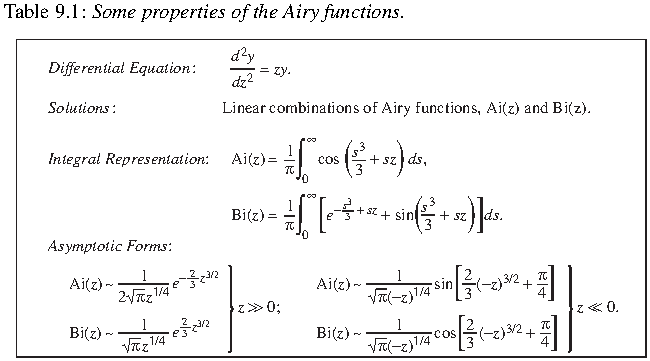
\includegraphics[width=1\linewidth]{./figures/airy-properties.pdf}
	\label{fig:Airy properties}
\end{figure}
